\chapter{Referencial Teórico}\label{cap:teo}
\section{Referencial e Rastreio de Satélites}\label{sec:ground_tracking}
Para iniciar a modelagem do sistema, é necessário descrever o referencial e entender como a estação de solo e o satélite se localizam no espaço.
Segundo \cite{soler1994}, utilizando um modelo esférico aproximado da Terra \ref{fig:modelagem_ang_visada} e sabendo a localização de latitude $\phi_S$ e longitude $\lambda_S$ da antena na estação, é possível estipular a direção em azimute e elevação para o apontamento da antena.
O raio da Terra para o modelo esférico será considerado de $R=6371 km$ e a distância do satélite em relação ao centro do modelo será considerada como $r = R+h$, com $h$ sendo a altitude de sua órbita.
Pode-se obter a longitude $\lambda_S$ na qual o vetor $\vec{r}$ intercepta a superfície da Terra, sendo possível traçar um triângulo reto esférico e utilizar a lei de Napier para obter a relação $\cos\gamma=\cos\phi_S\cos(\lambda_S-\lambda)$ \cite{soler1994}. Dessa forma, a distância entre o satélite e a estação de solo é dada pela equação \cite{soler1994}:
\begin{equation}
d = r[1+(R/r)^2-2(R/r)\cos\gamma]
\end{equation}
\begin{figure}[ht]
    \centering
    \caption{Modelagem matemática do ângulo de visada}
    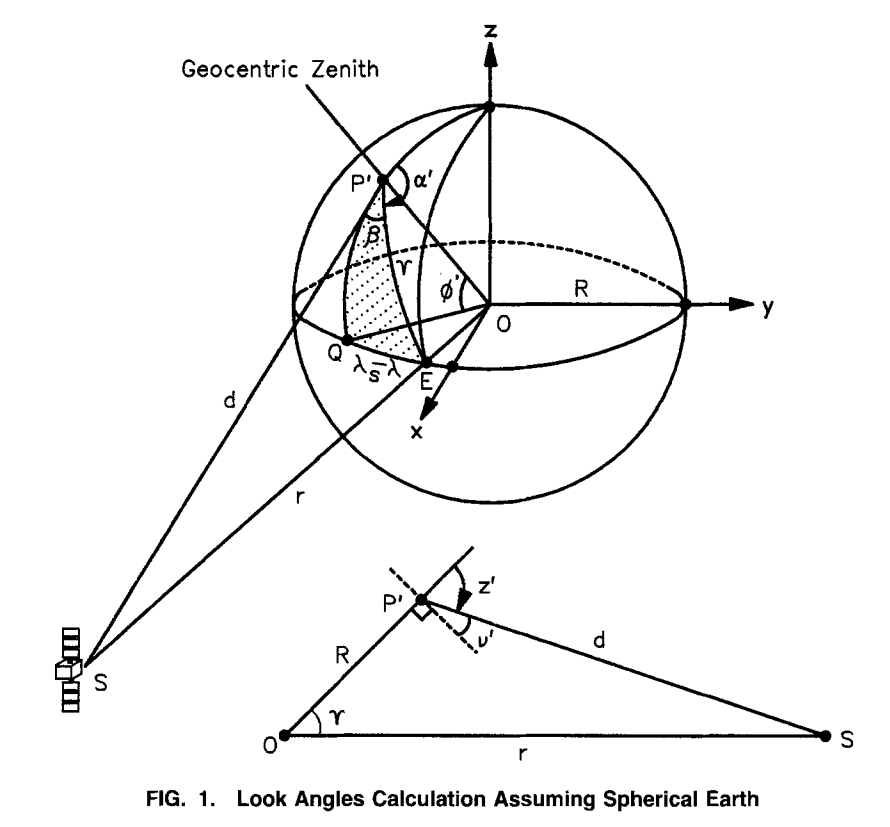
\includegraphics[width=0.8\textwidth]{figs/Interpretacao_geodesica.png}
    \legend{Fonte: \cite{soler1994}.}
    \label{fig:modelagem_ang_visada}
\end{figure}
A partir da equação anterior, é possível calcular a elevação $\nu_S$ e o azimute $\beta_S$ do satélite em relação à estação de solo a partir das seguintes equações:
\begin{align}
\nu_S = \arccos[(r/d)sin\gamma] \\
\beta_S = \arccos(\cot\gamma\tan\phi_S)
\end{align}
Essa modelagem foi feita considerando uma Terra esférica. Na realidade, a Terra possui uma forma aproximada de um elipsoide de revolução. Embora o modelo esférico ofereça uma aproximação inicial simples, ele introduz erros no cálculo do ângulo de elevação (ou distância zenital).
O formato faz com que o modelo esférico tenha algumas discrepâncias com as posições reais. No entanto, como o escopo do trabalho não é o modelo da Terra, mas sim o sistema de controle de apontamento da antena, bastará dizer que há a dedução de na literatura de \cite{soler1994} caso necessária a consulta.
Além disso, é esperado que os aplicativos com os quais o equipamento irá comunicar sejam baseados nos modelos mais completos, enviando a posição de azimute e elevação correta para o alinhamento com o satélite.

Podemos descrever o mecanismo apontamento da antena do pedestal a partir de dois movimentos independentes ortogonais, sendo um de azimute e um de elevação (sendo essa a configuração mais comum para mecanismos de apontamento).
O espaço de trabalho necessário para o acompanhamento contínuo de passagens de satélites corresponde ao hemisfério superior delimitado pelo horizonte local do plano tangente à estação de solo encontrado a 0$^\circ$ de elevação.
Para cobrir integralmente essa semi-esfera, o mecanismo deve ser capaz de efetuar uma rotação completa de $0$ até $2\pi$ (0$^\circ$ até 360$^\circ$) em azimute e uma articulação de $0$ até $\frac{\pi}{2}$ (0$^\circ$ até 90$^\circ$) na elevação.
Embora existam diversos mecanismos que tenham seu ângulo de elevação encurtado, já que em baixas elevações há a obstrução de relevo, estruturas ou atmosfera, o mecanismo desenvolvido nesse trabalho garantirá a varredura de toda região angular teórica.

É importante salientar que a partir das próximas modelagens as variáveis $\theta$ e $\phi$ serão também utilizadas ao se referir ao azimute e à elevação do mecanismo da antena.

\section{Modelagem do Pedestal}\label{sec:modelagem_pedestal}
Segundo \citeauthor{Ford2008}, o sistema pode ser modelado utilizando como base um manipulador esférico de dois graus de liberdade.
Utilizando o modelo pela figura \ref{fig:pedestal}, e utilizando como referência a modelagem de \cite{Bien2021} o ponto fixo que dará a referência do mecanismo com o solo será o da base, dado pelo referencial de coordenadas $O_0$, com versores $[x_0,y_0,z_0]$.
\begin{figure}[ht]
    \centering
    \caption{Modelo de pedestal com controle em azimute e elevação}
    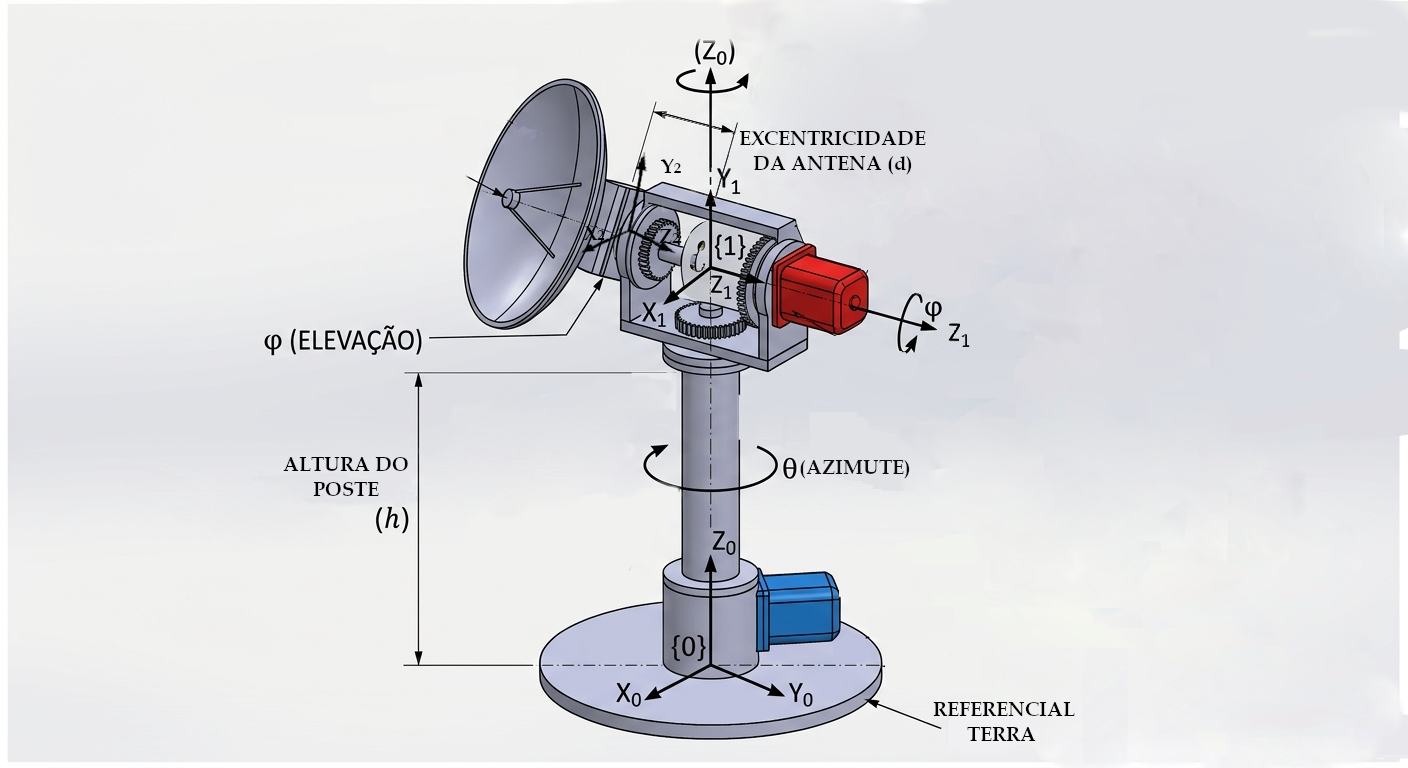
\includegraphics[width=0.8\textwidth]{figs/pedestal_proxy.png}
    \legend{Fonte: Elaborado pelo autor (2026).}
    \label{fig:pedestal}
\end{figure}
(TODO: explicar a localização dos motores)
Um motor é ligado por uma polia à base da antena, permitindo a rotação em torno do eixo Z. O ângulo de rotação do azimute é dado por $\theta$.
O segundo motor está localizado na região na qual a antena se encaixa ao poste do pedestal e é ligado ao eixo da elevação também através do mecanismo de polia. A junção da polia movida com o eixo da elevação tem coordenadas dadas pela origem $O_1$ ($[x_1,y_1,z_1]$) e distância da base dada pelo valor "h".
Além dos referenciais motorizados, será utilizando mais um referencial para descrever a excentricidade da antena, dado por $O_2$ ($[x_2,y_2,z_2]$) e distância de excentricidade "d"; e a região mais extrema que representa a ponta da antena, encontrada em  $O_3$ ($[x_3,y_3,z_3]$) e distância de braço "l".
O modelo da cinemática direta do sistema pode ser obtido a partir dos parâmetros de Denavit-Hatemberg (D-H). Utilizando como referenciais $O_i$ descrita pelos versores de referencial $[x_i,y_i,z_i]$ obtendo a tabela \ref{tab:params_d_h}
\begin{table}[ht]
\centering
\begin{tabular}{rrrrr}
    \hline
    Parâmetro & $\theta_i$ & $d_i$ & $a_i$ & $\alpha_i$ \\
    \hline
    $O_0O_1$ & $\theta$ & h & 0 & frac{$\pi$}{2} \\
    $O_1O_2$ & $\phi$ & -d & 0 & 0 \\
    $O_2O_3$ & 0 & 0 & l & 0 \\
\end{tabular}
\caption{Tabela de parâmetros D-H para o sistema}
\label{tab:params_d_h}
\end{table}

A partir da tabela D-H, a cinemática do sistema está completamente descrita e é possível determinar as matrizes de transformação homogênea de cada ponto utilizando o parâmetro \citeauthor{Siciliano2008}.
\begin{equation}
A^{i-1}_{i} = \begin{bmatrix}
\cos \theta_i & -\sin \theta_i \cos \alpha_i & \sin \theta_i \sin \alpha_i & a_i \cos \theta_i \\
\sin \theta_i & \cos \theta_i \cos \alpha_i & -\cos \theta_i \sin \alpha_i & a_i \sin \theta_i \\
0 & \sin \alpha_i & \cos \alpha_i & d_i \\
0 & 0 & 0 & 1
\end{bmatrix}
\end{equation}
Assim, é possível calcular como referenciais intermediários os seguintes pontos:
\begin{equation}
A^{0}_{1} = \begin{bmatrix}
\cos \theta & 0 & \sin \theta & 0 \\
\sin \theta & 0 & -\cos \theta & 0 \\
0 & 1 & 0 & h \\
0 & 0 & 0 & 1
\end{bmatrix}
\end{equation}
\begin{equation}
A^{1}_{2} = \begin{bmatrix}
\cos \phi & -\sin \phi & 0 & 0 \\
\sin \phi & \cos \phi & 0 & 0 \\
0 & 0 & 1 & -d \\
0 & 0 & 0 & 1
\end{bmatrix}
\end{equation}
\begin{equation}
A^{2}_{3} = \begin{bmatrix}
1 & 0 & 0 & l \\
0 & 1 & 0 & 0 \\
0 & 0 & 1 & 0 \\
0 & 0 & 0 & 1
\end{bmatrix}
\end{equation}
Utilizando a dedução de \cite{Siciliano2008}, pode-se computar a transformação homogênea de estado $T_{i}^{0} = A_{i}^{i-1} A_{i-1}^{i-2}(...)A_{1}^{0}$.
\begin{equation}
T^{0}_{1} = \begin{bmatrix}
\cos \theta & 0 & \sin \theta & 0 \\
\sin \theta & 0 & -\cos \theta & 0 \\
0 & 1 & 0 & h \\
0 & 0 & 0 & 1
\end{bmatrix}
\end{equation}
\begin{equation}
T^{0}_{2} = \begin{bmatrix}
\cos\theta\cos\phi - \sin\theta\sin\phi & -\cos\theta\sin\phi & \cos\theta\sin\phi+\sin\theta\cos\phi & \sin\theta(-\sin\phi) \\
\cos\theta\sin\phi + \sin\theta\cos\phi & \cos\theta\cos\phi & \sin\theta\sin\phi-\cos\theta\cos\phi & \sin\theta\cos\phi \\
0 & 1 & 0 & h-d \\
0 & 0 & 0 & 1
\end{bmatrix}
\end{equation}
\begin{equation}
T^{0}_{3} = \begin{bmatrix}
\cos\theta\cos\phi - \sin\theta\sin\phi & -\cos\theta\sin\phi & \cos\theta\sin\phi+\sin\theta\cos\phi & l-\sin\theta\sin\phi \\
\cos\theta\sin\phi + \sin\theta\cos\phi & \cos\theta\cos\phi & \sin\theta\sin\phi-\cos\theta\cos\phi & \sin\theta\cos\phi \\
0 & 1 & 0 & h-d \\
0 & 0 & 0 & 1
\end{bmatrix}
\end{equation}

\section{Estimação e Rastreio de Satélites}\label{sec:estimation}
Segundo a explicação de \cite{Ford2008}, cada satélite possui um número de catalogação que é utilizada para registrar informações básicas sobre a espaçonave. Embora algumas identificações (como nome e código de catalogação) são inalteradas durante sua vida útil, informações de órbita devem ser atualizadas constantemente por serem dinâmicas.
Agências como a North American Aerospace Defense Command (NORAD) e a National Aeronautics and Space Administration (NASA) utilizam radares e outras formas de medição para determinar a posição e órbita exata de satélites, mantendo um rastreio completo do céu.
Entre as métricas obtidas das observações estão os conhecidos elementos keplerianos. Esses elementos são informações como inclinação, excentricidade, decaimento de órbita, e perigeu.
A partir dos keplerianos, é possível estipular a posição do satélite no espaço em relação a um determinado tempo (passado ou futuro).
Softwares utilizam dessas informações para determinar passagens de diversos satélites e verificar quando estarão acima do horizonte, além de determinar o azimute e a elevação que a antena da estação de solo deverá ter para estar apontada para o satélite.
Apesar de possuir a posição (quase) exata dos satélites, os softwares de rastreio de satélites normalmente não têm uma taxa muito alta de atualização de envio de dados alta, sendo necessário um algoritmo para manter o rastreio durante os pontos sem informações novas.

Existem várias técnicas para a estimação da posição de um satélite ao longo do tempo. A primeira e mais simples é de enviar ao controlador dos motores a posição recebida do aplicativo e replicá-la na antena. O problema com esse método é que a estrutura sofre saltos grandes de posição, além de que a posição da antena ficará estática se o rotor perder a conexão com o software de rastreio.
Uma outra técnica é utilizar um filtro Kalman, que possui camadas de previsão e correção recursiva para fazer com que o Mínimo Erro Quadrático Médio seja nulo em relação a um modelo inicial. E o problema com o Filtro Kalman para esse caso é que ele é relativamente exigente em quesitos de processos, já que precisa recorrentemente atualizar as matrizes de ganhos.
Como é desejado que o projeto funcione completamente embarcado em um microcontrolador, esse tempo maior de processo pode causar demora no controle dos motores e fazer o sistema perder o rastreio do satélite. 
